%% FedFlow / FCHA paper, Springer Nature LaTeX template (sn-jnl), numbered references.
\documentclass[pdflatex,sn-mathphys-num]{sn-jnl}

\usepackage{graphicx}%
\usepackage{multirow}%
\usepackage{amsmath,amssymb,amsfonts}%
\usepackage{amsthm}%
\usepackage{mathrsfs}%
\usepackage[title]{appendix}%
\usepackage{xcolor}%
\usepackage{textcomp}%
\usepackage{manyfoot}%
\usepackage{booktabs}%
\usepackage{array}%

\newcommand{\best}[1]{\textbf{#1}}

\raggedbottom

\begin{document}

\title[Flow-Conditioned Host Attention for Federated IoT Intrusion Detection]{Flow-Conditioned Host Attention for Federated Intrusion Detection in IoT Networks: A Leakage-Controlled Evaluation on Unseen Traffic and Unseen Attackers}

\author*[1]{\fnm{First} \sur{Author}}\email{first.author@institution.edu}
\author[1]{\fnm{Second} \sur{Author}}\email{second.author@institution.edu}
\author[1]{\fnm{Third} \sur{Author}}\email{third.author@institution.edu}

\affil*[1]{\orgdiv{Department}, \orgname{Institution}, \orgaddress{\city{City}, \country{Country}}}

\abstract{Graph neural networks (GNNs) detect intrusions in network traffic by giving each connection (flow) information about the hosts it connects. Most of them describe a host by averaging all of its flows. In Internet of Things (IoT) networks a single machine often sends normal traffic and several kinds of attack at the same time, so this average is dominated by the most frequent traffic and a rare attack becomes hard to see. We propose Flow-Conditioned Host Attention (FCHA). For every flow it classifies, FCHA looks at the other flows of the sender and of the receiver and decides, using the flow itself as the attention query, which of them are relevant. FCHA is trained with federated learning: clients share model weights, feature statistics and validation counts, but never raw flows, labels or IP addresses. We evaluate it with a protocol designed to prevent data leakage: duplicated flows are capped, test sets contain either unseen traffic patterns or unseen attacker machines, every setting is repeated over 5 folds and 3 random seeds, and differences are tested with Holm-corrected Wilcoxon tests. On NF-ToN-IoT-v2, ToN-IoT-Network and NF-CSE-CIC-IDS2018-v2, FCHA is the best federated model on unseen traffic patterns, with 94.2\%, 99.1\% and 95.6\% balanced accuracy against 91.4\%, 98.6\% and 83.9\% for a centrally trained XGBoost ($p<0.001$), and it raises web-attack recall from at most 31.4\% to 80.4\%. Averaging host traffic, as recent federated GNN detectors do, costs up to 22 points. On unseen attacker machines all models drop sharply: FCHA has the best mean accuracy and the lowest false-positive rate on two datasets (6.0\% and 4.9\%), while a centrally trained random forest is best on the third.}

\keywords{Intrusion detection, Internet of Things, Federated learning, Graph neural networks, Attention, Data leakage}

\maketitle

\section{Introduction}\label{sec:intro}

Internet of Things (IoT) networks connect large numbers of small, often poorly protected devices. Network intrusion detection systems (NIDS) watch the traffic of these devices and raise an alert when a connection looks malicious. Modern NIDS learn this decision from labelled traffic. Good training data, however, is spread over many organisations, and they are rarely allowed to share it: flow records reveal internal addresses, running services and user behaviour. Federated learning (FL) solves this conflict by training one shared model while every organisation keeps its data on its own premises~\cite{mcmahan2017fedavg,kairouz2021advances}. FL has therefore become a common choice for IoT intrusion detection~\cite{nguyen2019diot,rahman2020iotids,campos2022evaluating,popoola2022zeroday}.

Network traffic has a natural graph structure. Hosts are the nodes, and every flow is a directed edge from a source host to a destination host. Graph neural networks (GNNs) use this structure to give each flow information about its surroundings~\cite{bilot2023survey,zhong2024survey}. E-GraphSAGE~\cite{lo2022egraphsage}, for example, summarises each host by aggregating the features of its flows, and classifies a flow from its own features plus the summaries of its two hosts. Federated detectors built on the same idea, such as FedGATSage~\cite{altfaily2025fedgatsage}, report accuracy close to centralised training.

\paragraph{The problem with averaging.} These models describe a host with one vector computed from \emph{all} of its flows. This works when a host sends only one kind of traffic. It fails when a host mixes traffic types, which is common in IoT testbeds. Consider an attacker machine that sends 1{,}000 benign flows, 1{,}000 injection flows and 20 backdoor flows. The average of its flows looks like benign or injection traffic. A backdoor flow from this machine therefore receives a host description that points to the wrong class, and the rare attack, which is the one a NIDS most needs to catch, becomes harder to detect.

\paragraph{The problem with evaluation.} Public NIDS benchmarks contain many exact duplicates. In NF-ToN-IoT-v2, keeping at most ten copies of each identical flow reduces the 16{,}809 backdoor flows to 239; in NF-CSE-CIC-IDS2018-v2 it reduces the 143{,}097 bot flows to 997. If flows are split at random, copies of the same record end up in both the training and the test set, and the test measures memory rather than detection. In addition, the few machines that generate an attack usually appear in both sets, so a model can learn to recognise the attacker instead of the attack. Such leakage is a known and recurring problem in machine learning for security~\cite{sommer2010closedworld,kaufman2012leakage,arp2022dos,engelen2021troubleshooting}, yet many federated GNN studies do not report how their test sets were built.

\paragraph{Contributions.} This paper addresses both problems:
\begin{enumerate}
\item \textbf{FCHA, a flow-conditioned aggregator.} Instead of one summary per host, every flow builds its own description of each endpoint. The flow under classification is the \emph{query} of an attention mechanism over the other flows of its sender and of its receiver, so it draws its context mainly from similar traffic (Section~\ref{sec:method}).
\item \textbf{A fully federated training pipeline.} Feature standardisation, model selection and model weights are all computed from aggregated client statistics. Raw flows, individual labels and IP addresses never leave a client (Section~\ref{sec:fed}).
\item \textbf{A leakage-controlled evaluation protocol.} We cap duplicates, test on unseen traffic patterns and on unseen attacker machines, check automatically that no feature reveals the label, verify that a model trained on shuffled labels scores at chance, and report 15 runs per setting with corrected significance tests (Section~\ref{sec:protocol}).
\item \textbf{A careful comparison on three benchmarks} against graph baselines that differ from FCHA only in how they aggregate, a federated flow-only network, and centrally trained tree ensembles, including an analysis of when host context helps and when it does not (Sections~\ref{sec:results} and \ref{sec:discussion}).
\end{enumerate}

\section{Related work}\label{sec:related}

\paragraph{Graph neural networks for intrusion detection.} GraphSAGE~\cite{hamilton2017graphsage} learns node representations by sampling and aggregating neighbours, and graph attention networks (GAT)~\cite{velickovic2018gat} weight neighbours with learned attention scores. In NIDS the informative features belong to the flows, that is, to the edges, so these node-level models need adapting. E-GraphSAGE~\cite{lo2022egraphsage} aggregates edge features into host embeddings and classifies each edge from the embeddings of its two endpoints. Chang and Branco~\cite{chang2024eres} add residual connections to this design and propose an attention-based variant, E-ResGAT, to cope with class imbalance. Anomal-E~\cite{caville2022anomale} trains edge embeddings without labels for anomaly detection, and Pujol-Perich et al.~\cite{pujolperich2022unveiling} show that a graph view of flows makes detection more robust to simple evasion attacks. Two recent surveys review the field~\cite{bilot2023survey,zhong2024survey}. In all of these models, a host's summary is the same for every flow that touches the host. In FCHA, by contrast, the summary depends on the flow being classified.

\paragraph{Federated intrusion detection.} Federated averaging (FedAvg)~\cite{mcmahan2017fedavg} trains a global model by repeatedly averaging locally updated weights. Its main difficulty is that clients hold differently distributed data~\cite{li2020flchallenges,kairouz2021advances}; label skew in particular slows training and lowers accuracy, and it is usually simulated by drawing each client's label proportions from a Dirichlet distribution~\cite{li2022noniid}. For IoT security, D\"IoT~\cite{nguyen2019diot} learns device-type-specific anomaly detectors federatedly, Rahman et al.~\cite{rahman2020iotids} compare centralised, on-device and federated training, Campos et al.~\cite{campos2022evaluating} evaluate federated detection on ToN-IoT under different data distributions, and Popoola et al.~\cite{popoola2022zeroday} use federated deep learning to detect zero-day botnet traffic. Graph-based federated detectors are more recent. FedGATSage~\cite{altfaily2025fedgatsage} runs graph attention on each client, groups nodes into communities, and sends community embeddings to a GraphSAGE model on the server; it reports 78.58\% balanced accuracy on NF-ToN-IoT. FedSTGCN~\cite{wang2025fedstgcn} combines spatial and temporal graph convolutions in a federated setting. Both rely on host-level or community-level aggregation, and neither describes a split that separates duplicate flows or attacker machines between training and test sets.

\paragraph{Datasets and evaluation.} Sarhan et al.~\cite{sarhan2022standard} converted several public datasets, including ToN-IoT~\cite{moustafa2021toniot} and CSE-CIC-IDS2018~\cite{sharafaldin2018cicids}, to a common NetFlow feature set, which makes results comparable across networks. Several works warn that NIDS results are easily inflated. Sommer and Paxson~\cite{sommer2010closedworld} explain why intrusion detection is harder than other learning tasks; Kaufman et al.~\cite{kaufman2012leakage} formalise data leakage; Arp et al.~\cite{arp2022dos} find leakage, sampling bias and weak baselines in many security papers; and Engelen et al.~\cite{engelen2021troubleshooting} report labelling and flow-construction errors in a widely used benchmark. We follow these recommendations: we remove duplicates across the split, hold out whole attacker machines, include strong tree-based baselines~\cite{breiman2001rf,chen2016xgboost}, and compare models with non-parametric paired tests~\cite{demsar2006statistical}.

\section{Problem setting}\label{sec:problem}

There are $K$ clients. Client $k$ owns a set of flows $\mathcal{E}_k$. A flow $e=(u,v,\mathbf{x}_e,y_e)$ goes from source host $u$ to destination host $v$, has a feature vector $\mathbf{x}_e\in\mathbb{R}^d$ (encoded NetFlow or Zeek fields) and a label $y_e\in\{1,\dots,C\}$, which is either \emph{benign} or one attack type. The flows of a client form a directed multigraph whose nodes are hosts. The task is to predict $y_e$ for every flow. IP addresses define the graph but are never used as features.

\paragraph{What is shared.} Clients never share flows, labels of individual flows or host addresses. They share model weights, aggregate feature statistics (count, sum and sum of squares of every feature) and aggregate validation confusion matrices. We assume an honest-but-curious server. We do not add formal privacy mechanisms such as differential privacy; Section~\ref{sec:discussion} discusses this limitation.

\paragraph{Inference.} A deployed model sees a window of unlabelled traffic. We therefore build the test graph only from test flows: when a test flow is classified, its context consists of other test flows, and no training flow or label is used.

\section{Flow-Conditioned Host Attention}\label{sec:method}

\begin{figure}[t]
\centering
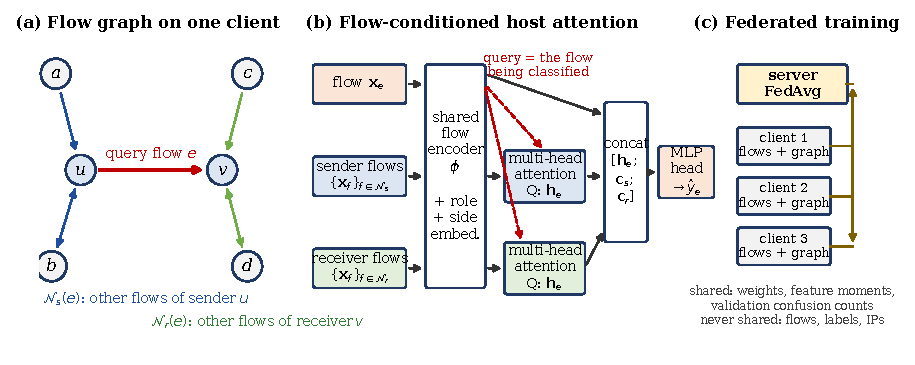
\includegraphics[width=\textwidth]{figures/fig_arch.pdf}
\caption{Overview of the approach. (a) The flow $e$ to classify goes from host $u$ to host $v$; both hosts have other flows. (b) FCHA encodes every flow with one shared encoder. It then attends over the sender's flows and, separately, over the receiver's flows, with the flow $e$ as the query. The flow's own embedding and the two resulting contexts are concatenated and classified. (c) Training is federated; only weights, feature statistics and validation counts are exchanged.}\label{fig:arch}
\end{figure}

Figure~\ref{fig:arch} gives an overview. All neural models in this paper share the same encoder, classifier, loss and training procedure. They differ only in how they build the context of a flow, so any difference in their results comes from the aggregation step.

\subsection{Flow encoder and neighbourhoods}\label{sec:encoder}

A shared encoder $\phi$ turns the features of a flow into a $D$-dimensional embedding, $\mathbf{h}_e=\phi(\mathbf{x}_e)$. $\phi$ is a two-layer perceptron with layer normalisation and a GELU activation.

For a flow $e$ from $u$ to $v$ we define two neighbourhoods. The \emph{sender neighbourhood} $\mathcal{N}_s(e)$ contains the other flows of host $u$, and the \emph{receiver neighbourhood} $\mathcal{N}_r(e)$ contains the other flows of host $v$, in both directions. Busy hosts can have thousands of flows, so we use at most $M$ of them: if a host has at most $M$ other flows we take all of them, otherwise we sample $M$ uniformly with replacement. The flow $e$ itself is never part of its own neighbourhood.

Each neighbour embedding receives two learned tags: whether the host was the sender or the receiver of that neighbour flow ($\boldsymbol{\rho}$), and whether it belongs to the sender or the receiver side of $e$ ($\boldsymbol{\sigma}$):
\begin{equation}
\tilde{\mathbf{h}}^{(t)}_f=\phi(\mathbf{x}_f)+\boldsymbol{\rho}_{\mathrm{role}(f)}+\boldsymbol{\sigma}_t,\qquad f\in\mathcal{N}_t(e),\; t\in\{s,r\}.\label{eq:tag}
\end{equation}

\subsection{Flow-conditioned attention}\label{sec:attention}

FCHA computes one context vector per side. The query comes from the flow being classified; the keys and values come from its neighbours. For side $t$ and each of $H$ attention heads (head index omitted for readability):
\begin{gather}
\mathbf{q}^{(t)} = \mathbf{W}_Q(\mathbf{h}_e+\boldsymbol{\sigma}_t),\qquad
\mathbf{k}^{(t)}_f = \mathbf{W}_K\tilde{\mathbf{h}}^{(t)}_f,\qquad
\mathbf{v}^{(t)}_f = \mathbf{W}_V\tilde{\mathbf{h}}^{(t)}_f, \label{eq:qkv}\\
\alpha^{(t)}_{ef} = \frac{\exp\!\big(\mathbf{q}^{(t)\top}\mathbf{k}^{(t)}_f/\sqrt{D/H}\big)}{\sum_{g\in\mathcal{N}_t(e)}\exp\!\big(\mathbf{q}^{(t)\top}\mathbf{k}^{(t)}_g/\sqrt{D/H}\big)}, \label{eq:att}\\
\mathbf{c}_t = \mathbf{W}_O\,\big\Vert_{h=1}^{H}\sum_{f\in\mathcal{N}_t(e)}\alpha^{(t,h)}_{ef}\,\mathbf{v}^{(t,h)}_f. \label{eq:ctx}
\end{gather}
This is scaled dot-product attention~\cite{vaswani2017attention}; $\Vert$ denotes concatenation of the heads. If a host has no other flow, its context is the zero vector. The class probabilities are
\begin{equation}
\hat{\mathbf{p}}_e=\operatorname{softmax}\!\big(\mathbf{W}_c\,\psi([\mathbf{h}_e;\mathbf{c}_s;\mathbf{c}_r])\big),\label{eq:out}
\end{equation}
where $\psi$ is a two-layer perceptron and $[\cdot\,;\cdot]$ is concatenation.

The weights $\alpha_{ef}$ in Eq.~\eqref{eq:att} depend on the query flow $e$. Two flows on the same host can therefore obtain very different contexts from it. In the example of Section~\ref{sec:intro}, a backdoor flow can put most of its attention on the few other backdoor flows of the machine, while a benign flow from the same machine attends to benign traffic. An average gives both flows the same, mostly benign, context.

\subsection{Baselines that differ only in aggregation}\label{sec:baselines}

Three baselines use exactly the same code and change one component:
\begin{itemize}
\item \textbf{E-GraphSAGE-mean} replaces the attention weights with uniform weights, $\alpha_{ef}=1/|\mathcal{N}_t(e)|$. The flow is classified from its own embedding and the mean context of each endpoint, as in E-GraphSAGE~\cite{lo2022egraphsage}.
\item \textbf{Host-mean} additionally removes $\mathbf{h}_e$ from Eq.~\eqref{eq:out}. The flow is classified only from the averages of its two hosts. This is the host-level aggregation used by federated GNN detectors such as FedGATSage~\cite{altfaily2025fedgatsage}.
\item \textbf{Flow-MLP} removes both contexts and classifies each flow from its own features only.
\end{itemize}

\subsection{Loss}\label{sec:loss}

We use cross-entropy with class weights. Each client computes the weights from its own class counts $n_c$ as $w_c\propto n_c^{-1/2}$ and scales them to an average of one. Square-root weighting gives rare classes more influence while avoiding the unstable training that full inverse-frequency weights cause on very rare classes~\cite{johnson2019imbalance,cui2019classbalanced}. In an ablation we also add a supervised contrastive term~\cite{khosla2020supcon} (weight 0.1, temperature 0.1).

\subsection{Fully federated training}\label{sec:fed}

Training follows FedAvg~\cite{mcmahan2017fedavg}. Three parts that are often done centrally are also federated:
\begin{itemize}
\item \textbf{Standardisation.} Every client sends the count, sum and sum of squares of each feature over its training flows. The server combines them into global means and standard deviations, which all clients and the test pipeline use. The result is identical to standardising the pooled data, but no raw value leaves a client.
\item \textbf{Model selection.} Each client keeps 10\% of its flows for validation. This hold-out is grouped by flow signature, so copies of a flow are never split between training and validation. After each round the clients evaluate the global model and send their confusion matrices; the server adds them up, computes balanced accuracy and keeps the best round. Training stops after 10 rounds without improvement.
\item \textbf{Weights.} In each round every client trains for one local epoch (at most 600 steps, batch size 512, AdamW, learning rate $3\times10^{-4}$, weight decay $10^{-4}$, gradient clipping at 5). The server averages the client weights in proportion to their training-set sizes. Training runs for at most 30 rounds.
\end{itemize}

\subsection{Cost}\label{sec:cost}

Because every neighbourhood has at most $M$ flows, classifying a flow costs $O(MD)$ operations no matter how many flows its hosts have. With $D=128$, $H=4$ and $M=16$, FCHA has 171{,}000 parameters (0.68\,MB in 32-bit floats). E-GraphSAGE-mean has 121{,}000, Host-mean 105{,}000 and Flow-MLP 72{,}000. In each round, a client downloads and uploads one copy of the weights.

\section{Evaluation protocol}\label{sec:protocol}

\subsection{Datasets}\label{sec:data}

Table~\ref{tab:datasets} lists the three benchmarks. NF-ToN-IoT-v2 and NF-CSE-CIC-IDS2018-v2 are the NetFlow versions~\cite{sarhan2022standard} of ToN-IoT~\cite{moustafa2021toniot} and CSE-CIC-IDS2018~\cite{sharafaldin2018cicids}. ToN-IoT-Network is the original ToN-IoT network training and testing set, which contains Zeek connection, DNS, HTTP and SSL fields. From the two large NetFlow datasets we read at most 150{,}000 flows per class; smaller classes are kept in full. As in the base study~\cite{altfaily2025fedgatsage}, we drop the ransomware and man-in-the-middle classes of ToN-IoT. The 15 original labels of CSE-CIC-IDS2018 are merged into 7 attack families. NF-ToN-IoT-v2 and ToN-IoT-Network were recorded on the same testbed and share attacker machines; NF-CSE-CIC-IDS2018-v2 comes from an independent network.

\begin{table}[t]
\caption{Datasets after duplicate capping (at most 10 copies of each identical flow). Features are counted after encoding.}\label{tab:datasets}
\begin{tabular*}{\textwidth}{@{\extracolsep\fill}lrrcc}
\toprule
Dataset & Flows read & Flows after capping & Classes & Features \\
\midrule
NF-ToN-IoT-v2 & 1{,}066{,}809 & 396{,}551 & 8 & 158 \\
ToN-IoT-Network & 190{,}000 & 130{,}248 & 8 & 153 \\
NF-CSE-CIC-IDS2018-v2 & 833{,}872 & 280{,}632 & 7 & 148 \\
\botrule
\end{tabular*}
\end{table}

\subsection{Features and leakage checks}\label{sec:features}

Numeric fields are transformed with $\operatorname{sign}(x)\log(1+|x|)$. We add three derived features (byte and packet asymmetry, bytes per packet, byte rate), group port numbers into well-known, registered and ephemeral ranges, and one-hot encode categorical fields using vocabularies learned from training data only. Labels, the binary attack flag, flow identifiers and IP addresses are never used as features. An automatic check rejects any column whose values determine the label on the training data. This check matters in practice: in an earlier version of our pipeline, a label-index column left among the features produced 93\% balanced accuracy on random-noise data.

\subsection{Duplicate capping}\label{sec:dups}

Capping keeps only 37\% of the NF-ToN-IoT-v2 flows and 34\% of the NF-CSE-CIC-IDS2018-v2 flows, and some classes are far more repetitive (backdoor: 16{,}809 flows reduced to 239; bot: 143{,}097 reduced to 997). We keep at most 10 copies of each identical flow before any split. Without this step the folds were badly unbalanced; one NF-CSE-CIC-IDS2018-v2 test fold consisted of 66\% bot flows and contained only 9 brute-force flows.

\subsection{Two test scenarios}\label{sec:splits}

\paragraph{Unseen traffic patterns (signature split).} The \emph{signature} of a flow is the tuple of destination port, protocol, inbound and outbound bytes, inbound and outbound packets, and duration. We use 5-fold stratified group cross-validation with the signature as the group. No test flow therefore has an identical copy in its training set; we verified that every fold has zero signature overlap.

\paragraph{Unseen attackers (leave-attacker-out split).} An \emph{attacker host} is any source of at least 50 attack flows. We distribute the attacker hosts over 5 folds, starting with the busiest and always adding the next one to the fold with the fewest attack flows; all other hosts are assigned at random. A test fold contains every flow sent by its hosts, and none of these flows appears in training. The model must therefore detect attacks from machines it has never seen. A class whose only attacker is in the test fold cannot be learned, so on this split we compute balanced accuracy over the \emph{supported} classes, i.e.\ those with at least 50 test flows that also occur in training. Table~\ref{tab:attackerfolds} shows what each fold tests on ToN-IoT-Network.

A plain $K$-fold split over all source hosts does not work on these benchmarks. Each attack type is produced by only a handful of machines among hundreds of hosts, so most folds would contain no attack. In a trial on NF-ToN-IoT-v2, three of five such folds had between 4 and 865 test flows and no attack at all.

\begin{table}[t]
\caption{Leave-attacker-out folds on ToN-IoT-Network. For each fold: the held-out attacker machine and the attack classes in its test set (number of training flows of the same class, from other machines, in brackets).}\label{tab:attackerfolds}
\begin{tabular*}{\textwidth}{@{\extracolsep\fill}cl>{\raggedright\arraybackslash}p{0.62\textwidth}}
\toprule
Fold & Attacker & Attack classes tested \\
\midrule
F0 & 192.168.1.30 & DDoS 14{,}215 (2{,}647); DoS 18{,}578 (1{,}296); injection 7{,}813 (12{,}081); password 8{,}609 (9{,}124); scanning 5{,}910 (6{,}862) \\
F1 & 192.168.1.31 & DDoS 2{,}643 (14{,}219); DoS 603 (19{,}271); injection 12{,}080 (7{,}814); password 9{,}124 (8{,}609); scanning 1{,}974 (10{,}798) \\
F2 & 192.168.1.32 & scanning 4{,}888 (7{,}884); XSS 8{,}275 (537) \\
F3 & 192.168.1.193 & backdoor 6{,}817 (143) \\
F4 & 4 minor hosts & backdoor 143; DoS 692; XSS 537 \\
\botrule
\end{tabular*}
\end{table}

\subsection{Clients, models and baselines}\label{sec:setup}

The training data are split over $K=5$ clients, either at random (IID) or with label skew drawn from a Dirichlet distribution with $\alpha=0.5$ (at least 200 flows per client)~\cite{li2022noniid}. FCHA and Flow-MLP are trained under both settings, the graph baselines under IID. Each client builds its graph only from its own flows. FCHA uses $D=128$, $H=4$, $M=16$ and dropout 0.1.

As strong non-graph references we train a random forest (200 trees)~\cite{breiman2001rf} and XGBoost (300 trees, depth 8, learning rate 0.1)~\cite{chen2016xgboost} on the same features. These two models are trained \emph{centrally} on the pooled data, an advantage the federated models do not have; tables mark them with $\dagger$. Two ablations are run on the signature split: FCHA with the supervised contrastive term, and FCHA trained centrally (one client).

\subsection{Metrics and statistical tests}\label{sec:metrics}

The main metric is balanced accuracy, the mean recall over classes, which is not dominated by large classes. We also report macro-F1 and the false-positive rate (FPR), the share of benign flows flagged as attacks. Each setting is run on all 5 folds with seeds 42, 43 and 44, giving 15 runs, and we report mean $\pm$ sample standard deviation. To compare a model with FCHA we apply the two-sided Wilcoxon signed-rank test~\cite{wilcoxon1945} to the 15 paired (fold, seed) results, as recommended for comparing classifiers~\cite{demsar2006statistical}, and correct the $p$-values within each table with Holm's method~\cite{holm1979}. As a sanity check, FCHA is also trained once per fold on randomly shuffled labels; it must score at chance level.

\subsection{Implementation}\label{sec:impl}

The pipeline is written in PyTorch and scikit-learn. Graph models were trained mostly on NVIDIA T4 GPUs and partly on CPUs. Each run is identified by a hash of every setting that affects its result, so runs from different machines can be merged without duplicates.

\section{Results}\label{sec:results}

\begin{figure}[t]
\centering
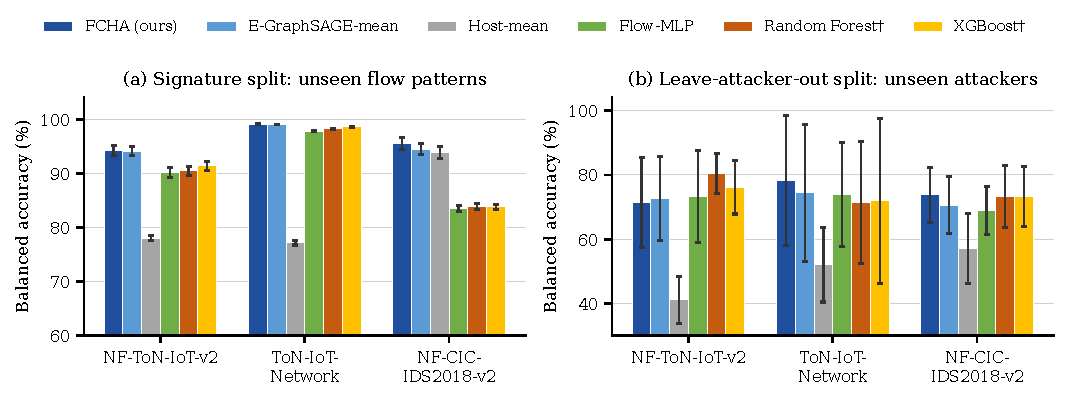
\includegraphics[width=\textwidth]{figures/fig_main.pdf}
\caption{Balanced accuracy (mean $\pm$ standard deviation over 5 folds $\times$ 3 seeds, IID clients) on (a) unseen traffic patterns and (b) unseen attackers. $\dagger$: trained centrally.}\label{fig:main}
\end{figure}

\subsection{Unseen traffic patterns}\label{sec:res-sig}

Table~\ref{tab:signature} and Fig.~\ref{fig:main}(a) show the signature split. FCHA has the highest balanced accuracy on all three datasets (tied with E-GraphSAGE-mean on ToN-IoT-Network). It is significantly better than Flow-MLP and both tree ensembles on every dataset ($p<0.001$). The gap is largest on NF-CSE-CIC-IDS2018-v2: 95.6\% for FCHA against 83.9\% for both centrally trained tree models and 83.5\% for Flow-MLP. ToN-IoT-Network is almost saturated: every model except Host-mean exceeds 97.7\%, and FCHA leads XGBoost by 0.5 points.

Mean aggregation (E-GraphSAGE-mean) is close to FCHA on the two ToN-IoT datasets and 1.1 points behind on NF-CSE-CIC-IDS2018-v2 ($p<0.001$). Host-mean, which ignores the flow's own features, behaves very differently across datasets. It loses 16.2 and 21.9 points on NF-ToN-IoT-v2 and ToN-IoT-Network, and on NF-ToN-IoT-v2 it flags 31.0\% of benign flows as attacks. On NF-CSE-CIC-IDS2018-v2 it is only 1.7 points behind. The reason is the structure of the data. In CSE-CIC-IDS2018 most attacker machines run a single attack type, so a host's average identifies its attack. In ToN-IoT the attacker machines mix several attack types with benign traffic, and the average hides them. This is exactly the situation that motivates FCHA.

For reference, FedGATSage reports 78.58\% balanced accuracy on NF-ToN-IoT~\cite{altfaily2025fedgatsage}. Our Host-mean baseline, which uses the same kind of host-level aggregation, reaches 78.0\% on NF-ToN-IoT-v2 under our protocol, and FCHA reaches 94.2\%. The dataset version and the split differ, so this comparison is indicative only.

\begin{table}[t]
\caption{Unseen traffic patterns (signature split), IID clients. Mean $\pm$ standard deviation over 15 runs. BA: balanced accuracy; F1: macro-F1; FPR: false-positive rate (all in \%). $p$: Holm-corrected Wilcoxon test against FCHA. $\dagger$: trained centrally. Best value per dataset in bold.}\label{tab:signature}
\begin{tabular*}{\textwidth}{@{\extracolsep\fill}lcccc}
\toprule
Model & BA & F1 & FPR & $p$ \\
\midrule
\multicolumn{5}{l}{\emph{NF-ToN-IoT-v2}}\\
FCHA (ours) & \best{94.2} $\pm$ 0.9 & \best{92.2} $\pm$ 1.5 & 4.6 $\pm$ 0.3 & -- \\
E-GraphSAGE-mean & 94.1 $\pm$ 0.9 & 92.0 $\pm$ 1.7 & 4.5 $\pm$ 0.4 & 0.095 \\
Host-mean & 78.0 $\pm$ 0.5 & 74.9 $\pm$ 1.5 & 31.0 $\pm$ 1.0 & $<$0.001 \\
Flow-MLP & 90.1 $\pm$ 0.9 & 87.2 $\pm$ 2.2 & 6.7 $\pm$ 0.8 & $<$0.001 \\
Random forest$\dagger$ & 90.5 $\pm$ 0.8 & 91.1 $\pm$ 0.8 & \best{3.5} $\pm$ 0.3 & $<$0.001 \\
XGBoost$\dagger$ & 91.4 $\pm$ 0.9 & 91.7 $\pm$ 0.8 & 4.8 $\pm$ 0.4 & $<$0.001 \\
\midrule
\multicolumn{5}{l}{\emph{ToN-IoT-Network}}\\
FCHA (ours) & \best{99.1} $\pm$ 0.1 & \best{99.1} $\pm$ 0.1 & \best{0.1} $\pm$ 0.1 & -- \\
E-GraphSAGE-mean & \best{99.1} $\pm$ 0.1 & 99.0 $\pm$ 0.1 & \best{0.1} $\pm$ 0.1 & 0.008 \\
Host-mean & 77.2 $\pm$ 0.4 & 76.9 $\pm$ 0.4 & 0.2 $\pm$ 0.1 & $<$0.001 \\
Flow-MLP & 97.8 $\pm$ 0.1 & 97.4 $\pm$ 0.1 & 0.7 $\pm$ 0.1 & $<$0.001 \\
Random forest$\dagger$ & 98.3 $\pm$ 0.1 & 98.3 $\pm$ 0.1 & 0.3 $\pm$ 0.1 & $<$0.001 \\
XGBoost$\dagger$ & 98.6 $\pm$ 0.1 & 98.6 $\pm$ 0.1 & 0.4 $\pm$ 0.1 & $<$0.001 \\
\midrule
\multicolumn{5}{l}{\emph{NF-CSE-CIC-IDS2018-v2}}\\
FCHA (ours) & \best{95.6} $\pm$ 1.1 & \best{90.2} $\pm$ 0.4 & \best{2.9} $\pm$ 0.2 & -- \\
E-GraphSAGE-mean & 94.5 $\pm$ 1.1 & \best{90.2} $\pm$ 0.4 & 3.1 $\pm$ 0.4 & $<$0.001 \\
Host-mean & 93.9 $\pm$ 1.2 & 89.4 $\pm$ 0.4 & 4.8 $\pm$ 0.6 & $<$0.001 \\
Flow-MLP & 83.5 $\pm$ 0.6 & 85.2 $\pm$ 0.6 & 11.1 $\pm$ 2.8 & $<$0.001 \\
Random forest$\dagger$ & 83.9 $\pm$ 0.6 & 83.8 $\pm$ 0.5 & 10.4 $\pm$ 0.7 & $<$0.001 \\
XGBoost$\dagger$ & 83.9 $\pm$ 0.5 & 86.1 $\pm$ 0.6 & 6.5 $\pm$ 0.4 & $<$0.001 \\
\botrule
\end{tabular*}
\end{table}

\subsection{Rare attack classes}\label{sec:res-class}

Table~\ref{tab:perclass} lists recall per class. FCHA's advantage comes mostly from rare classes and from classes whose flows look like other traffic. On NF-CSE-CIC-IDS2018-v2, web attacks (only 1{,}520 flows after capping) are recognised with 80.4\% recall by FCHA, 72.8\% by mean aggregation and at most 31.4\% by any flow-only model. Infiltration recall rises from at most 69.9\% to 98.6\%. On NF-ToN-IoT-v2, backdoor recall rises from 77.3--81.2\% (flow-only models) to 92.8\%. The one class where FCHA is behind is DDoS on NF-CSE-CIC-IDS2018-v2 (92.8\% against 99.9\% for Flow-MLP and XGBoost). The confusion matrix in Fig.~\ref{fig:confusion} shows where these errors go: 7\% of DDoS flows are predicted as web attacks and 19\% of web flows as DDoS. The remaining mistakes are thus confusions between two attack types, not missed attacks, and FCHA has the highest benign recall (97.1\%) of all models.

\begin{table}[t]
\caption{Recall per class (\%), signature split, mean over 15 runs. EGS: E-GraphSAGE-mean; MLP: Flow-MLP; RF and XGB: random forest and XGBoost, trained centrally ($\dagger$).}\label{tab:perclass}
\begin{tabular*}{\textwidth}{@{\extracolsep\fill}lccccc}
\toprule
Class & FCHA & EGS & MLP & RF$\dagger$ & XGB$\dagger$ \\
\midrule
\multicolumn{6}{l}{\emph{NF-CSE-CIC-IDS2018-v2}}\\
Benign & \best{97.1} & 96.9 & 88.9 & 89.6 & 93.5 \\
DDoS & 92.8 & 94.0 & \best{99.9} & 97.1 & \best{99.9} \\
Infiltration & \best{98.6} & 98.0 & 68.0 & 69.9 & 66.0 \\
Web & \best{80.4} & 72.8 & 28.6 & 31.4 & 27.6 \\
Bot, brute force, DoS & $\geq$99.9 & $\geq$99.9 & $\geq$99.1 & $\geq$99.1 & $\geq$99.9 \\
\midrule
\multicolumn{6}{l}{\emph{NF-ToN-IoT-v2}}\\
Backdoor & \best{92.8} & 92.2 & 81.2 & 77.3 & 80.0 \\
Injection & \best{86.7} & \best{86.7} & 77.0 & 84.8 & 85.0 \\
Password & \best{89.5} & 89.4 & 87.4 & 84.7 & 87.6 \\
XSS & \best{93.9} & 93.5 & 89.7 & 88.4 & 89.8 \\
DoS & \best{99.8} & \best{99.8} & 98.4 & 98.0 & 98.6 \\
Benign & 95.4 & 95.5 & 93.3 & \best{96.5} & 95.2 \\
\botrule
\end{tabular*}
\end{table}

\begin{figure}[t]
\centering
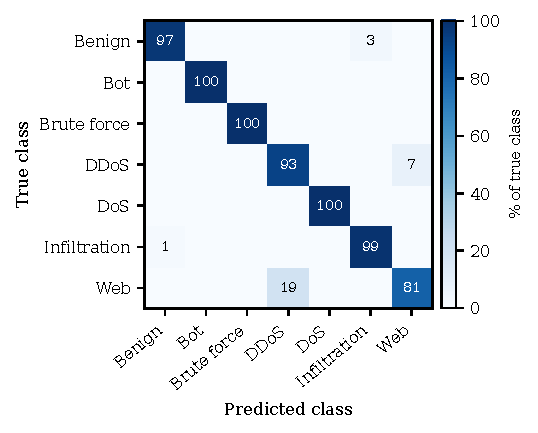
\includegraphics[width=0.55\textwidth]{figures/fig_confusion_cic.pdf}
\caption{Confusion matrix of FCHA on NF-CSE-CIC-IDS2018-v2 (signature split), summed over 15 runs and normalised per true class.}\label{fig:confusion}
\end{figure}

\subsection{Unseen attackers}\label{sec:res-att}

Table~\ref{tab:attacker} and Fig.~\ref{fig:attacker} show the leave-attacker-out split. This scenario is much harder for every model. Compared with the signature split, FCHA loses 21--23 points of balanced accuracy and the tree ensembles 10--27 points. Results also vary strongly from fold to fold (standard deviations of 6--26 points), more than most differences between models.

\begin{itemize}
\item \textbf{ToN-IoT-Network.} FCHA has the highest mean (78.3\%), ahead of E-GraphSAGE-mean (74.5\%), Flow-MLP (74.0\%) and both tree ensembles (71.4\% and 71.9\%). It also has the lowest false-positive rate (6.0\% against 11.2--22.1\%). The largest gain is in fold F2, where the main XSS attacker is unseen and only 537 XSS flows from other machines are available for training: FCHA reaches 90.6\%, Flow-MLP 70.8\% and the trees 66.0--67.7\%. Fold F3 holds out the only backdoor attacker, leaving 143 backdoor training flows from other machines, and every model fails on it (28.2--49.3\%).
\item \textbf{NF-CSE-CIC-IDS2018-v2.} FCHA (73.8\%) is level with the trees (73.3\%) and has the lowest false-positive rate (4.9\%, against 6.3\% for XGBoost and 10.8\% for the random forest).
\item \textbf{NF-ToN-IoT-v2.} The centrally trained random forest is best (80.3\% against 71.4\% for FCHA, $p=0.041$). FCHA's deficit comes almost entirely from fold F2, in which backdoor, password and scanning attackers are held out; its recall on these classes falls below 12\%.
\end{itemize}

Apart from Host-mean, which is significantly worse everywhere, the only significant differences to FCHA on this split are Flow-MLP on NF-CSE-CIC-IDS2018-v2 (worse, $p=0.017$) and the random forest on NF-ToN-IoT-v2 (better, $p=0.041$).

\begin{table}[t]
\caption{Unseen attackers (leave-attacker-out split), IID clients. BA is computed over supported classes. Mean $\pm$ standard deviation over 15 runs; columns as in Table~\ref{tab:signature}.}\label{tab:attacker}
\begin{tabular*}{\textwidth}{@{\extracolsep\fill}lcccc}
\toprule
Model & BA & F1 & FPR & $p$ \\
\midrule
\multicolumn{5}{l}{\emph{NF-ToN-IoT-v2}}\\
FCHA (ours) & 71.4 $\pm$ 14.1 & 72.5 $\pm$ 16.0 & 11.8 $\pm$ 9.3 & -- \\
E-GraphSAGE-mean & 72.7 $\pm$ 13.1 & 73.9 $\pm$ 14.3 & 19.1 $\pm$ 17.7 & 0.757 \\
Host-mean & 41.1 $\pm$ 7.3 & 39.7 $\pm$ 8.4 & 64.2 $\pm$ 15.7 & $<$0.001 \\
Flow-MLP & 73.4 $\pm$ 14.3 & 70.9 $\pm$ 17.6 & 16.3 $\pm$ 14.5 & 0.757 \\
Random forest$\dagger$ & \best{80.3} $\pm$ 6.2 & \best{77.8} $\pm$ 7.7 & \best{10.5} $\pm$ 12.1 & 0.041 \\
XGBoost$\dagger$ & 76.2 $\pm$ 8.4 & 70.5 $\pm$ 15.0 & 12.1 $\pm$ 12.8 & 0.757 \\
\midrule
\multicolumn{5}{l}{\emph{ToN-IoT-Network}}\\
FCHA (ours) & \best{78.3} $\pm$ 20.2 & \best{78.6} $\pm$ 19.5 & \best{6.0} $\pm$ 9.1 & -- \\
E-GraphSAGE-mean & 74.5 $\pm$ 21.4 & 74.9 $\pm$ 18.9 & 11.2 $\pm$ 18.2 & 0.428 \\
Host-mean & 52.0 $\pm$ 11.6 & 54.4 $\pm$ 12.3 & 20.1 $\pm$ 25.7 & $<$0.001 \\
Flow-MLP & 74.0 $\pm$ 16.2 & 72.1 $\pm$ 17.3 & 17.0 $\pm$ 26.1 & 0.428 \\
Random forest$\dagger$ & 71.4 $\pm$ 19.0 & 71.1 $\pm$ 17.1 & 16.5 $\pm$ 25.5 & 0.428 \\
XGBoost$\dagger$ & 71.9 $\pm$ 25.6 & 74.4 $\pm$ 22.5 & 22.1 $\pm$ 26.5 & 0.428 \\
\midrule
\multicolumn{5}{l}{\emph{NF-CSE-CIC-IDS2018-v2}}\\
FCHA (ours) & \best{73.8} $\pm$ 8.5 & \best{71.1} $\pm$ 8.8 & \best{4.9} $\pm$ 2.4 & -- \\
E-GraphSAGE-mean & 70.5 $\pm$ 8.8 & 66.5 $\pm$ 13.0 & 5.0 $\pm$ 3.0 & 0.321 \\
Host-mean & 57.2 $\pm$ 10.9 & 52.3 $\pm$ 15.1 & 6.4 $\pm$ 4.4 & $<$0.001 \\
Flow-MLP & 68.8 $\pm$ 7.5 & 63.3 $\pm$ 11.8 & 13.8 $\pm$ 6.2 & 0.017 \\
Random forest$\dagger$ & 73.3 $\pm$ 9.7 & 70.4 $\pm$ 11.3 & 10.8 $\pm$ 1.1 & 0.338 \\
XGBoost$\dagger$ & 73.3 $\pm$ 9.4 & 65.5 $\pm$ 17.7 & 6.3 $\pm$ 1.8 & 0.762 \\
\botrule
\end{tabular*}
\end{table}

\begin{figure}[t]
\centering
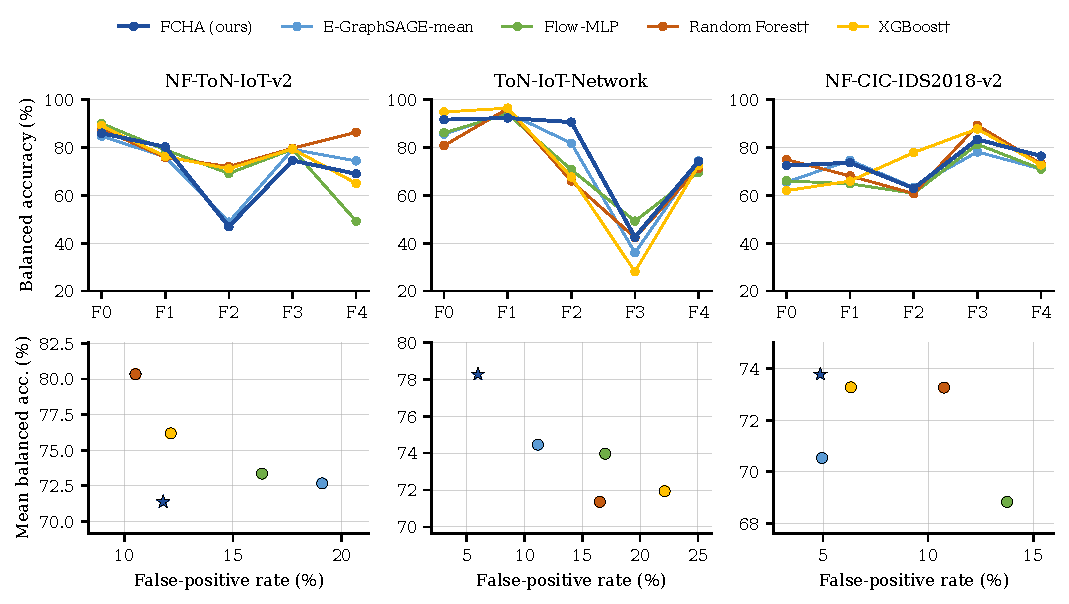
\includegraphics[width=\textwidth]{figures/fig_attacker.pdf}
\caption{Unseen attackers. Top: balanced accuracy per fold (mean of 3 seeds); each fold holds out different attacker machines. Bottom: mean balanced accuracy against false-positive rate over all 15 runs; FCHA is marked with a star, and the upper left corner is best.}\label{fig:attacker}
\end{figure}

\subsection{Cost of federation and ablations}\label{sec:res-abl}

Table~\ref{tab:ablation} separates the effect of federation from the effect of the model. With IID clients, federated FCHA is within 0.3 points of centrally trained FCHA on every dataset; the 0.1-point gap on ToN-IoT-Network is statistically significant but negligible in practice. Label-skewed (Dirichlet) clients cost FCHA 1.1, 0.1 and 2.0 points, more than they cost Flow-MLP on two datasets, yet FCHA with skewed clients still beats every flow-only model, including the centrally trained trees. The supervised contrastive term has no measurable effect ($p\geq0.28$), so the final model does not use it.

\begin{table}[t]
\caption{Cost of federation and ablations on the signature split: balanced accuracy (\%), mean over 15 runs. All variants are federated over 5 clients except the centrally trained one ($\dagger$). NF-CIC-IDS2018-v2: NF-CSE-CIC-IDS2018-v2.}\label{tab:ablation}
\begin{tabular*}{\textwidth}{@{\extracolsep\fill}lccc}
\toprule
Variant & NF-ToN-IoT-v2 & ToN-IoT-Network & NF-CIC-IDS2018-v2 \\
\midrule
FCHA, IID clients & 94.2 & 99.1 & 95.6 \\
FCHA, Dirichlet(0.5) clients & 93.1 & 99.0 & 93.6 \\
FCHA, centrally trained$\dagger$ & 94.5 & 99.2 & 95.6 \\
FCHA + contrastive loss, IID & 94.0 & 99.1 & 95.6 \\
\midrule
Flow-MLP, IID clients & 90.1 & 97.8 & 83.5 \\
Flow-MLP, Dirichlet(0.5) clients & 89.6 & 97.6 & 83.0 \\
\botrule
\end{tabular*}
\end{table}

\subsection{What the attention looks at}\label{sec:res-lift}

To check the mechanism directly, we measure the \emph{attention lift} on hosts whose flows belong to at least two classes. For query flows of class $c$ on such hosts, we divide the attention weight that FCHA places on same-class neighbours by the share of same-class neighbours, which is the weight a plain average would give them. A lift above one means that attention concentrates on similar traffic. Labels are used only for this analysis, after training.

Table~\ref{tab:lift} shows that the lift depends on the class. On NF-CSE-CIC-IDS2018-v2 it is highest for web attacks (1.58), the class with the largest gain over mean aggregation (80.4\% against 72.8\% recall), and for bot traffic (1.37). On both ToN-IoT datasets it is highest for DoS (1.89 and 1.66). On the unseen-attacker split of NF-CSE-CIC-IDS2018-v2 it stays well above one for bot (2.03), DDoS (1.56) and brute force (1.42). For several frequent classes the lift is close to or below one, so attention does not single out same-class traffic for every class; the mechanism should be understood per class, not as a general property.

\begin{table}[t]
\caption{Attention lift of FCHA on hosts with mixed classes (signature split, mean over runs). Values above 1 mean that attention favours flows of the same class. NF-CIC-v2: NF-CSE-CIC-IDS2018-v2; NF-ToN-v2: NF-ToN-IoT-v2; ToN-Network: ToN-IoT-Network.}\label{tab:lift}
\begin{tabular}{@{}lc@{\hspace{2.2em}}lc@{\hspace{2.2em}}lc@{}}
\toprule
\multicolumn{2}{c}{NF-CIC-v2} & \multicolumn{2}{c}{NF-ToN-v2} & \multicolumn{2}{c}{ToN-Network} \\
\cmidrule(lr){1-2}\cmidrule(lr){3-4}\cmidrule(lr){5-6}
Web & \best{1.58} & DoS & \best{1.89} & DoS & \best{1.66} \\
Bot & 1.37 & DDoS & 1.28 & Password & 1.34 \\
DoS & 1.02 & Scanning & 1.18 & Scanning & 1.00 \\
Infiltration & 0.99 & Password & 1.08 & XSS & 0.94 \\
Benign & 0.97 & Benign & 0.90 & Benign & 0.91 \\
DDoS & 0.96 & XSS & 0.79 & DDoS & 0.75 \\
\botrule
\end{tabular}
\end{table}

\subsection{Communication and sanity checks}\label{sec:res-comm}

A complete FCHA run (about 26--28 rounds with 5 clients) exchanges 199--205\,MB in total, compared with 143--146\,MB for E-GraphSAGE-mean and 80--86\,MB for Flow-MLP. Per client and round this is 1.4\,MB. Feature statistics and confusion matrices add only a few kilobytes. Every run on shuffled labels scored at chance level (12.5\% balanced accuracy with 8 classes and 14.3\% with 7), which confirms that no feature or preprocessing step leaks the label.

\section{Discussion}\label{sec:discussion}

\paragraph{When does flow-conditioned context help?} The results show two different regimes. When the traffic pattern or the attacking machine has been seen during training, endpoint context is very informative, and how it is aggregated matters. Averaging alone hurts when hosts mix classes (ToN-IoT) and is harmless when they do not (CSE-CIC-IDS2018). On this split, flow-conditioned attention is never worse than mean aggregation and is clearly better on rare classes. When the attacker is new, the endpoint context describes a machine the model has never seen. It still helps when the new attack resembles traffic from other attackers (ToN-IoT-Network, fold F2). It fails when a class has almost no training examples from other machines (fold F3) or when several classes are held out together (NF-ToN-IoT-v2, fold F2).

\paragraph{Fewer false alarms.} On two of the three datasets, FCHA reaches its unseen-attacker accuracy with the lowest false-positive rate of all models: 6.0\% against 16.5--22.1\% for the tree ensembles on ToN-IoT-Network, and 4.9\% against 6.3--10.8\% on NF-CSE-CIC-IDS2018-v2. Security analysts must inspect every alert, so a detector with similar detection and fewer false alarms is preferable in practice. On NF-ToN-IoT-v2 this advantage does not hold (11.8\% against 10.5\% for the random forest).

\paragraph{Lessons for evaluation.} Two observations apply beyond our model. First, duplicate capping and signature grouping change the conclusions: before capping, one of our test folds was two-thirds bot traffic and per-class results were unstable. Second, accuracy drops by 10--27 points (21--23 for FCHA) between the signature split and the leave-attacker-out split. Results on random or signature splits therefore say little about how a detector will behave against new attacking machines, and we recommend reporting both scenarios.

\paragraph{Limitations.} (i) NF-ToN-IoT-v2 and ToN-IoT-Network come from the same testbed, so the study covers two independent networks; more testbeds would strengthen the conclusions. (ii) The clients are simulated partitions of one dataset; real sites would have different hosts and traffic mixes. (iii) We use FedAvg without differential privacy or secure aggregation. Shared weights can leak information, and the accuracy cost of such protections for FCHA is still to be measured. (iv) The test graph is built from a batch of traffic; a streaming deployment would need graphs over time windows. (v) The tree ensembles are trained centrally; federated tree learning would make the comparison fully symmetric.

\section{Conclusion}\label{sec:conclusion}

We introduced FCHA, a graph model for federated IoT intrusion detection in which every flow attends to the flows of its two hosts and uses itself as the query. We evaluated it under a protocol that controls data leakage: duplicates are capped, test sets contain either unseen traffic patterns or unseen attacker machines, and every setting is repeated 15 times with corrected significance tests. On unseen traffic patterns, FCHA is the best federated model on all three benchmarks, improves the recall of rare attacks by up to 52 points over flow-only models, and loses nothing against centralised training when clients are IID. Host-level averaging, common in federated GNN detectors, loses up to 22 points. On unseen attackers, the hardest and most realistic scenario, FCHA is competitive with centrally trained tree ensembles and raises clearly fewer false alarms on two of three datasets, but it does not win everywhere. Letting the model learn when to trust host context, and adding formal privacy guarantees, are the main directions for future work.

\backmatter

\bmhead{Acknowledgements}
[To be completed by the authors.]

\section*{Declarations}

\begin{itemize}
\item \textbf{Funding:} [To be completed by the authors.]
\item \textbf{Competing interests:} The authors declare no competing interests. [Confirm.]
\item \textbf{Ethics approval and consent to participate:} Not applicable; the study uses only public, anonymised network-traffic datasets.
\item \textbf{Consent for publication:} Not applicable.
\item \textbf{Data availability:} The datasets are publicly available from their original providers~\cite{sarhan2022standard,moustafa2021toniot,sharafaldin2018cicids}. The per-run result records behind every table and figure are available at [repository URL].
\item \textbf{Code availability:} The code and all configuration files are available at [repository URL].
\item \textbf{Author contributions:} [To be completed by the authors, e.g.\ using the CRediT taxonomy.]
\item \textbf{Use of AI tools:} [Describe any use of AI-assisted tools in preparing this manuscript, as required by the journal's editorial policy.]
\end{itemize}

\bibliography{refs}

\end{document}
